\documentclass[]{article}
\usepackage{hyperref}
\usepackage{amsmath}
\usepackage[style=nature]{biblatex}
\usepackage{geometry}
\usepackage{graphicx}
\usepackage{subfig}

\geometry{margin=0.65in}

\bibliography{Hanabi.bib}

\title{Solving Hanabi with Neural Network}
\author{Ciruzzi Michele}

\begin{document}

\maketitle

% Abstract (short summary, few lines) 
\begin{abstract}
	Try to exploit a board game with incomplete and asymmetric information is not simple, as stated in a paper \cite{BARD2020103216} that I read too late. Nevertheless I've tried to solve it, obviously failing. This report will show (some of) the lessons I've learnt. 
\end{abstract}

\section{Problem}
Hanabi is a cooperative game for 2 to 5 players with incomplete and asymmetric information.
Because of this features it has been proposed by DeepMind group \parencite{BARD2020103216} as a new challenge for Reinforcement learning.
The problem has been tackled both with deterministic (e.g \cite{Cox2015}) and ML-learning based algorithms (e.g. \cite{Lerer2019}).
The game has been demonstrated to be NP-Hard in general \parencite{Baffier2016}.
As a rule of thumb a good algorithm is able to consistently achieve 20 or more points (out of 25).
My aim is to train a neural network which can achieve a good score in playing Hanabi using a Deep-Q Learning algorithm \cite{Mnih2015} (like the \textit{Rainbow} policy in \cite{BARD2020103216}).
The code used for the last attempts can be found in the zip file attached or in the master branch of \url{https://github.com/TnTo/Hanabi/}, while some of the first attempts are available in the other branches (particularly v0.2, v0.3, v0.4). The notebooks in the folder are written to work on CoLab.

% Methods
\section{Methods}
Even if more sophisticated algorithms are available, I have implemented the Deep-Q-Learning algorithm introduced by \textcite{Mnih2015}.
As far as I know, the source code used in the paper is not available and not every step of the algorithm is explained in detail, so there are some differences between the algorithm presented in the paper and my implementation (in particular, I simulated the result of each action applied onto the observed state, instead of estimating the unobserved actions with the neural network, which resulted in a bottleneck in my code).
I implemented the algorithm from scratch using keras and numpy, which has critically improved the performance compared with a previous pure python implementation. 
The algorithm can be summarized as follows:
\begin{enumerate}
	\item Play some games performing random actions to populate the memory
	\item Select a subset of the memories, calculate the target value of each action for each board state in memory (see below) and then train the network
	\item Initialize a given number of new games and retrieve some board states from the memory, play these games with a given policy (see below) until they end, adding to the memory each board state observed
	\item repeat steps 2 and 3, playing some new games after the step 2 to test the ability of the network to improve the achieved score in subsequent iterations.
\end{enumerate}
The target value for step 2 is
$$Q(s_t, a_t) = score(s_{t+1} | s_t, a_t) - score(s_t) + \gamma \max_{a_{t+1} \in actions} Q(s_{t+1}, a_{t+1})$$
where $s_t$ is the board state at time $t$ and $a_t$ is the action performed. $\gamma$ is a discount factor used to account for long-term outlook. The values computed in step 2 were cut into the interval $[0,\frac{1-\gamma^{max score}}{1-\gamma}]$ which are the only possible values of $Q$ for how the game works.
The policy used in step 3 is the following: with probability $\epsilon$ the action is chosen randomly, otherwise $argmax_{a_t \in actions} Q(s_t, a_t)$ is chosen.
In fact, the learning goal is to approximate $Q$ as well as possible with a neural network.
For the neural network a MSE loss and a RMSProp optimizer have been used (as in \cite{Mnih2015}) with different leaning rates (generally between $10^{-2}$ and $10^{-4}$), numbers of hidden layers (from 1 to 3), number of neurons (from 32 to 1024) and activations (sigmoid, tanh, ReLU and PReLU has been tried). 
The dimension of the output layer is equal to the number of different actions available. An early stopping mechanism was used, with a sensibility of 0.01 and a waiting time of 100 epochs.
The three metrics I've monitored are the minimum loss in each training round (step 2), the points achieved in the test play (step 4) and the predicted values of $Q$ for the memories after each learning round (step 2).

%Results
\section{Results}
\subsection{Gradient saturation}
In an early implementation the output layer had a single neuron, i.e estimated $Q(s_t, a_t)$ passing both $s_t$ and $a_t$ as input, and the network used to saturate the gradient pretty fast. The solution was using a PReLU or Leaky ReLU activation. The problem vanished when I switched to a n-dimensional output layer.

\subsection{LR sensibility}
This problem needs a very small learning rate to converge ($10^{-4}$ or less, as in \cite{Mnih2015}).
An example of the predicted values of $Q$ with a learning rate of $10^2$ is displayed in figure 1.
On the other hand with a small learning rate the network shows slow to null improvement and can still diverge in the long run.
An improvement could come from a more adaptive optimizer or a dynamical correction of the learning rate.

\subsection{Sensibility to initialization}
Another element which produces instability, slows down convergence and reduces accuracy is the network initialization.
A random uniform initializer was used initially with large interval ($[-1,1]$), and later on with a smaller interval ($[-10^{-4}, 10^{4}]$) which solved the issue. The predicted values of $Q$ for the first case are displayed in figure 2.

\subsection{Q saturation}
The formula for updating $Q$ leads to $\max |Q| \propto (k\gamma)^t$, which grows unlimited if some predictions are big enough (figure 3), while the theoretical maximum of $Q$ is $\frac{1-\gamma^{max score}}{1-\gamma}$. Cutting target values to $[0,\frac{1-\gamma^{max score}}{1-\gamma}]$ interval keeps the grow in check but creates a saturation around the upper bound of the interval (figure 4). Additionally a lower $\gamma$ (0.5) reduces the saturation but also the agent's foresight.

\subsection{Reducing the dimensionality}
Another attempt to simplify the problem was the dimensionality reduction of the environment and actions space (by reducing the number of players, colours and numbers and providing complete information to the agents).
Anyway it has not led to any drastic improvement.

%Conclusion/Future Development
\section{Conclusions}
Deep Q-Learning is an elegant and conceptually simple algorithm for reinforcement learning but it requires fine tuning and, probably, a very long training time.
Improvements could came from different angles:
\begin{itemize}
	\item review the literature and adopt one of the already developed Hanabi simulators \cite{BARD2020103216}
	\item adopt some of the improved variants of Deep-Q Learning already proposed (e.g. \cite{vanhasselt2015deep})
	\item tweak the optimizer, network dimension and learning rate
	\item change the data flow in term of games played, replayed and memory selection (possibly introducing asynchronous computing)
	\item introduce a convolutional layer and/or a recurrent network structure
	\item use genetic algorithms to preserve the black-box approach
	\item create (or find in literature, e.g. \cite{Lerer2019}) an ad-hoc reinforce learning algorithm which keeps into account the rules of the game. To do this a starting point could be the deterministic algorithms already proposed in literature (e.g. \cite{Cox2015}).
\end{itemize}


\begin{figure}[t]
	\centering
	\begin{tabular}{cc}
		\subfloat[predicted $Q$ values for high (0.01) learning rate]{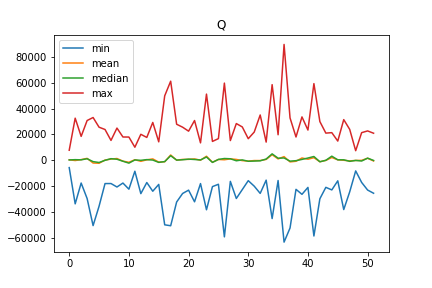
\includegraphics[width=0.45\linewidth]{../LearningRate/Qs.png}} &
		\subfloat[predicted $Q$ values for {[-1,1]} random uniform initialization of weights]{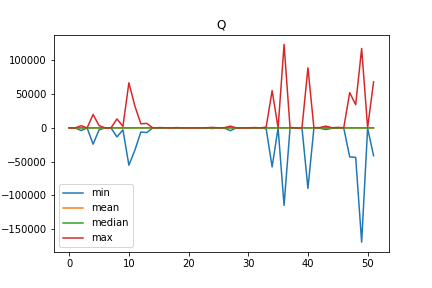
\includegraphics[width=0.45\linewidth]{../Initialization/Qs.png}} \\
		\subfloat[predicted $Q$ values for high (0.95) $\gamma$ without cutting]{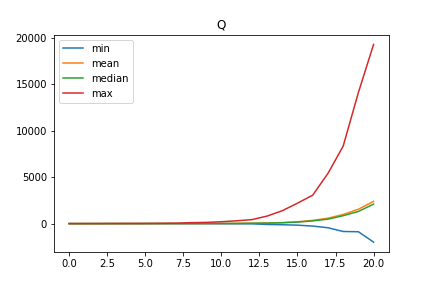
\includegraphics[width=0.45\linewidth]{../QUnlimited/Qs.png}} &
		\subfloat[predicted $Q$ values for high (0.95) $\gamma$ with cutting]{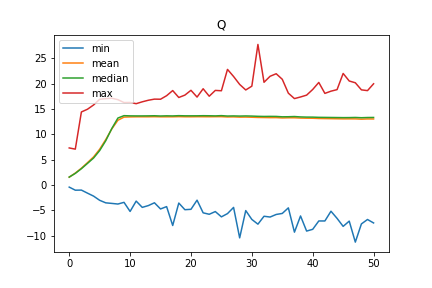
\includegraphics[width=0.45\linewidth]{../QFeedback/Qs.png}} \\
	\end{tabular}
\end{figure}

\printbibliography{}

\end{document}


